\PassOptionsToPackage{hidelinks}{hyperref}
\documentclass[11pt,letterpaper]{article}

\usepackage[utf8]{inputenc}
\usepackage[T1]{fontenc}
\usepackage[spanish,es-tabla]{babel}
\usepackage{lmodern}
\usepackage{microtype}

\usepackage[letterpaper,margin=2.3cm]{geometry}
\usepackage{setspace}
\setstretch{1.08}

\usepackage{xcolor}
\usepackage{graphicx}
\usepackage{float}
\usepackage{caption}
\usepackage{amsmath,amssymb}
\usepackage{booktabs}
\usepackage{tabularx}
\usepackage{array}
\usepackage{enumitem}
\usepackage{titlesec}
\usepackage{tcolorbox}
\tcbuselibrary{breakable}
\usepackage{tikz}
\usetikzlibrary{arrows.meta,positioning,shapes.geometric,calc}
\usepackage{pgfplots}
\pgfplotsset{compat=1.18}
\usepackage{hyperref}

\definecolor{principal}{HTML}{1F4E79}
\definecolor{secundario}{HTML}{2F7D6D}
\definecolor{acento}{HTML}{B85C38}
\definecolor{fondo}{HTML}{F6F8FA}
\definecolor{borde}{HTML}{D8DEE9}
\definecolor{textoSuave}{HTML}{4A5568}

\hypersetup{
    colorlinks=true,
    linkcolor=principal,
    urlcolor=principal,
    citecolor=principal
}

\titleformat{\section}
    {\Large\bfseries\color{principal}}
    {}
    {0pt}
    {}
    [\titlerule]

\titleformat{\subsection}
    {\large\bfseries\color{secundario}}
    {}
    {0pt}
    {}

\titleformat{\subsubsection}
    {\normalsize\bfseries\color{textoSuave}}
    {}
    {0pt}
    {}

\titlespacing*{\section}{0pt}{1.2em}{0.7em}
\titlespacing*{\subsection}{0pt}{1em}{0.45em}
\titlespacing*{\subsubsection}{0pt}{0.8em}{0.35em}

\setlist[itemize]{leftmargin=1.3em,itemsep=0.25em,topsep=0.35em}
\setlist[enumerate]{leftmargin=1.5em,itemsep=0.25em,topsep=0.35em}

\newtcolorbox{nota}{
    breakable,
    colback=fondo,
    colframe=borde,
    boxrule=0.6pt,
    arc=2mm,
    left=3mm,
    right=3mm,
    top=2mm,
    bottom=2mm
}

\newcommand{\code}[1]{\texttt{\detokenize{#1}}}
\newcommand{\dato}[2]{\textbf{#1:} #2}
\newcommand{\important}[1]{\textbf{\color{principal}#1}}

\newcolumntype{Y}{>{\raggedright\arraybackslash}X}
\newcolumntype{L}[1]{>{\raggedright\arraybackslash}p{#1}}

\pgfplotsset{
    every axis/.append style={
        axis line style={borde},
        tick style={borde},
        tick label style={font=\small},
        label style={font=\small},
        title style={font=\bfseries\small},
        scaled ticks=false,
        yticklabel style={/pgf/number format/fixed},
        xticklabel style={/pgf/number format/fixed},
        grid=major,
        grid style={draw=borde!55},
    }
}


\begin{document}

\pagenumbering{gobble}
\begin{titlepage}
    \centering
    \vspace*{0.35cm}

    \begin{tabularx}{\textwidth}{>{\centering\arraybackslash}m{2.8cm}
        >{\centering\arraybackslash}X
        >{\centering\arraybackslash}m{2.8cm}}
        
\includegraphics[height=2.55cm]{figures/escudo_unam.png}
        &
        \begin{minipage}{0.56\textwidth}
            \centering
            {\Large\bfseries Universidad Nacional Autónoma de México\par}
            \vspace{0.18cm}
            {\large Facultad de Ciencias\par}
        \end{minipage}
        &
        
\includegraphics[height=2.55cm]{figures/escudo_facultad_ciencias.png}
    \end{tabularx}

    \vspace{0.5cm}
    {\color{principal}\rule{0.72\textwidth}{0.8pt}\par}
    \vspace{0.35cm}
    {\large\bfseries Almacenes y Minería de Datos\par}
    {\normalsize Semestre 2026-2\par}
    \vspace{0.35cm}
    {\color{principal}\rule{0.72\textwidth}{0.8pt}\par}

    \vfill

    {\Huge\bfseries\color{principal} Proyecto final\par}
    \vspace{0.45cm}
    {\LARGE Reporte formal\par}

    \vfill

    \begin{minipage}{0.92\textwidth}
        \begin{nota}
            \begin{tabularx}{\textwidth}{L{2.8cm}Y}
                \textbf{Profesora:} & Jessica Santizo Galicia \\
                \textbf{Ayudante:} & Diego Antonio Villalba González \\
                \textbf{Ayud. Lab.:} & Ares Gael Castro Romero \\
            \end{tabularx}
        \end{nota}

        \vspace{0.45cm}

        \begin{nota}
            \centering
            \textbf{Alumnos}\\[0.25cm]
            Omar Fernando Gramer Muñoz\\
            Kevin Steve Quezada Ordoñez\\
            Jesús Antonio Romero Godoy\\
            Edgar Salgado González
        \end{nota}
    \end{minipage}

    \vspace{0.85cm}
    {\large Junio de 2026\par}
\end{titlepage}

\clearpage
\pagenumbering{arabic}

\section*{1. Introducción}

\begin{nota}
Para el desarrollo del proyecto se seleccionó el dataset
\code{atus_anual_2024.csv}, el cual registra los accidentes de tránsito
terrestre registrados durante 2024. El dataset contiene 390,627
registros y 45 variables

La información permite caracterizar cada accidente a partir de elementos como su
ubicación, fecha y hora, tipo de percance, vehículos involucrados, posible causa, características del conductor y número de personas heridas o
fallecidas. Esta variedad de atributos ofrece una base adecuada para aplicar
técnicas de análisis y minería de datos a lo largo del proyecto.
\end{nota}

\section*{2. Tema, problema y justificación}

\begin{nota}
\dato{Área temática}{Transporte y movilidad.}

\vspace{0.45em}
\textbf{1. ¿Cuál es el problema?}

Los accidentes de tránsito terrestre en zonas urbanas y suburbanas de México
representan un problema de movilidad y seguridad pública por su frecuencia y por
la variedad de consecuencias que generan. El fenómeno se acota al año 2024 y al
estudio de su severidad: accidentes con sólo daños materiales, accidentes no
fatales y accidentes fatales. El punto central es distinguir qué condiciones del
evento, del lugar, del momento, de los vehículos involucrados y del conductor
presunto responsable se relacionan con consecuencias de mayor gravedad.

\vspace{0.6em}
\textbf{2. ¿Por qué es relevante?}

Su relevancia es social y económica. Social, porque los accidentes afectan de
forma directa la integridad de conductores, pasajeros, peatones y ciclistas, y 
económica porque incluso los eventos sin víctimas implican daños materiales,
interrupciones en la movilidad y costos para personas, aseguradoras e
instituciones públicas. En 2024 se identifican 374,949 accidentes reales después
de separar los registros administrativos sin percance. De ellos, 306,841 se
clasifican como sólo daños, 63,920 como no fatales y 4,188 como fatales. En
conjunto, los registros reportan 85,980 personas heridas y 4,656 personas
fallecidas, cifras suficientes para considerar el fenómeno como un problema
significativo dentro del área de transporte y movilidad.

\vspace{0.6em}
\textbf{3. ¿Qué se busca lograr?}

El objetivo es identificar patrones medibles que ayuden a diferenciar la
severidad de los accidentes de tránsito. En términos concretos, se busca
reconocer qué combinaciones de zona, temporalidad, tipo de percance, vehículos
involucrados, causa presunta, superficie de rodamiento y características del
conductor aparecen con mayor frecuencia en cada nivel de severidad. Esto permite
caracterizar perfiles de accidentes y distinguir los eventos con sólo daños de
aquellos que involucran personas heridas o fallecidas.

\vspace{0.6em}
\textbf{4. ¿Por qué este dataset?}

El archivo \code{atus_anual_2024.csv} es pertinente porque proviene de una fuente
oficial, pública y verificable, y describe una problemática real y vigente en
México. Contiene 390,627 registros y 45 variables con cobertura municipal. Sus
columnas incluyen información geográfica, temporal, categórica y numérica:
ubicación del evento, tipo de accidente, zona urbana o suburbana, vehículos
involucrados, causa presunta, superficie de rodamiento, características del
conductor y conteos de personas heridas o fallecidas. Además, la variable
\code{CLASACC} clasifica directamente la severidad del accidente, lo que permite
plantear análisis supervisado, al mismo tiempo, la variedad de atributos
descriptivos permite formar grupos de accidentes con características similares.
\end{nota}


\section*{3. Datos utilizados}

\begin{nota}
El dataset seleccionado forma parte del programa \textit{Accidentes de Tránsito
Terrestre en Zonas Urbanas y Suburbanas} (ATUS), publicado por el Instituto
Nacional de Estadística y Geografía (INEGI). Los datos pueden descargarse
desde la página oficial:

\begin{center}
    \url{https://www.inegi.org.mx/programas/accidentes/?ps=Microdatos#datos_abiertos}
\end{center}

\vspace{0.25em}
Dentro del apartado de microdatos se utilizó la opcion de 
\textit{Accidentes de tránsito terrestre en zonas urbanas y suburbanas,
1997--2024}. El archivo comprimido (\code{.zip}) disponible en esa sección incluye la
siguiente estructura general:

\begin{itemize}
    \item \code{catalogos/}: catálogos auxiliares de día, edad, entidad, hora,
    minuto, municipio y mes.
    \item \code{conjunto_de_datos/}: archivos anuales correspondientes al
    periodo 1997--2024.
    \item \code{diccionario_de_datos/}: descripción de las variables utilizadas.
    \item \code{metadatos/}: información complementaria sobre el conjunto.
    \item \code{leeme_faq.txt}: notas y preguntas frecuentes.
\end{itemize}

Para este proyecto se seleccionó \code{atus_anual_2024.csv}, ya que es el
archivo anual más reciente incluido en la descarga y permite analizar el estado
actual del problema.

\vspace{0.25em}
\begin{tabularx}{\textwidth}{L{4.1cm}Y}
    \toprule
    \textbf{Requisito} & \textbf{Justificación} \\
    \midrule
    Datos reales relacionados con México
        & Los registros provienen de INEGI y están relacionados con accidentes
          de tránsito ocurridos en zonas urbanas y suburbanas del país durante
          2024. \\
    Volumen mínimo
        & El archivo \code{atus_anual_2024.csv} contiene 390,627 filas y 45
          columnas, por encima del mínimo de 100,000 registros y 8 variables
          relevantes. \\
    Variables numéricas y categóricas
        & Incluye variables numéricas, como el número de vehículos, personas
          heridas y fallecidas, y variables categóricas, como el tipo de
          accidente, la causa presunta, el día de la semana y la clasificación
          del evento. \\
    Fuente pública, verificable y citable
        & El conjunto se obtiene desde el portal oficial de datos abiertos del
          INEGI, mediante la liga indicada anteriormente. \\
    Modelado supervisado y agrupamiento
        & La variable \code{CLASACC} permite plantear tareas de clasificación
          según la severidad del accidente. A su vez, los atributos temporales,
          geográficos, vehiculares y del conductor permiten agrupar registros
          con características similares. \\
    \bottomrule
\end{tabularx}
\end{nota}

\newpage
\section*{4. Diccionario oficial de datos}

\begin{nota}
El archivo \code{diccionario_de_datos_atus_anual_2024.csv}, publicado junto con
los datos del INEGI, documenta las 45 columnas del dataset original. A
continuación se presenta una versión resumida de sus descripciones oficiales.
Las variables se agrupan por su función para facilitar la lectura, pero se
conservan sus nombres y tipos de dato originales.

\vspace{0.4em}
Los valores permitidos y las definiciones extensas permanecen disponibles en el
diccionario oficial. En particular, deben considerarse los códigos especiales
que representan información no especificada, conductores fugados o registros
administrativos con valor \code{Certificado cero}.
\end{nota}

\subsection*{4.1 Identificación, localización y tiempo}

\begin{nota}
\small
\begin{tabularx}{\textwidth}{L{3cm}L{1.45cm}Y}
    \toprule
    \textbf{Variable} & \textbf{Tipo} & \textbf{Descripción resumida} \\
    \midrule
    \code{COBERTURA} & \code{varchar} & Área geográfica a la que se refieren los indicadores. \\
    \code{ID_ENTIDAD} & \code{varchar} & Clave INEGI de la entidad federativa. \\
    \code{ID_MUNICIPIO} & \code{varchar} & Clave INEGI del municipio, debe interpretarse junto con la entidad. \\
    \code{ANIO} & \code{int} & Año en el que ocurrió el accidente. \\
    \code{MES} & \code{varchar} & Mes de referencia del accidente. \\
    \code{ID_HORA} & \code{int} & Hora del accidente, el código 99 indica hora no especificada. \\
    \code{ID_MINUTO} & \code{int} & Minuto del accidente, el código 99 indica minuto no especificado. \\
    \code{ID_DIA} & \code{varchar} & Día del mes, el código 32 indica día no especificado. \\
    \code{DIASEMANA} & \code{varchar} & Día de la semana en que ocurrió el evento. \\
    \code{URBANA} & \code{varchar} & Tipo de ubicación dentro de una zona urbana. \\
    \code{SUBURBANA} & \code{varchar} & Tipo de vía o camino dentro de una zona suburbana. \\
    \bottomrule
\end{tabularx}
\end{nota}

\subsection*{4.2 Características del accidente y del conductor}

\begin{nota}
\small
\begin{tabularx}{\textwidth}{L{3cm}L{1.45cm}Y}
    \toprule
    \textbf{Variable} & \textbf{Tipo} & \textbf{Descripción resumida} \\
    \midrule
    \code{TIPACCID} & \code{varchar} & Tipo de percance, como colisión, volcadura, salida del camino o incendio. \\
    \code{CAUSAACCI} & \code{varchar} & Causa presunta registrada para el accidente. \\
    \code{CAPAROD} & \code{varchar} & Tipo de superficie de rodamiento: pavimentada o no pavimentada. \\
    \code{SEXO} & \code{varchar} & Sexo registrado del conductor presunto responsable. \\
    \code{ALIENTO} & \code{varchar} & Registro de aliento alcohólico del conductor. \\
    \code{CINTURON} & \code{varchar} & Uso registrado de cinturón de seguridad por parte del conductor. \\
    \code{ID_EDAD} & \code{varchar} & Edad del conductor, 0 indica fuga y 99 edad desconocida. \\
    \bottomrule
\end{tabularx}
\end{nota}

\newpage
\subsection*{4.3 Vehículos involucrados}

\begin{nota}
\small
Las siguientes columnas numéricas indican cuántos vehículos de cada categoría
participaron en el accidente.

\vspace{0.4em}
\begin{tabularx}{\textwidth}{L{3cm}L{1.45cm}Y}
    \toprule
    \textbf{Variable} & \textbf{Tipo} & \textbf{Descripción resumida} \\
    \midrule
    \code{AUTOMOVIL} & \code{int} & Automóviles de hasta siete asientos. \\
    \code{CAMPASAJ} & \code{int} & Camionetas de pasajeros de 8 a 15 asientos. \\
    \code{MICROBUS} & \code{int} & Microbuses de 16 a 20 asientos. \\
    \code{PASCAMION} & \code{int} & Camiones urbanos de pasajeros de 21 a 29 asientos. \\
    \code{OMNIBUS} & \code{int} & Ómnibus de 30 o más asientos. \\
    \code{TRANVIA} & \code{int} & Trenes eléctricos o trolebuses. \\
    \code{CAMIONETA} & \code{int} & Camionetas destinadas al transporte de carga. \\
    \code{CAMION} & \code{int} & Camiones destinados al transporte de carga. \\
    \code{TRACTOR} & \code{int} & Tractores con o sin remolque. \\
    \code{FERROCARRI} & \code{int} & Ferrocarriles involucrados. \\
    \code{MOTOCICLET} & \code{int} & Motocicletas involucradas. \\
    \code{BICICLETA} & \code{int} & Bicicletas involucradas. \\
    \code{OTROVEHIC} & \code{int} & Otros vehículos no incluidos en las categorías anteriores. \\
    \bottomrule
\end{tabularx}
\end{nota}

\subsection*{4.4 Víctimas, severidad y publicación}

\begin{nota}
\small
Las variables de víctimas contabilizan personas fallecidas o heridas según su
forma de participación en el accidente.

\vspace{0.4em}
\begin{tabularx}{\textwidth}{L{3cm}L{1.45cm}Y}
    \toprule
    \textbf{Variable} & \textbf{Tipo} & \textbf{Descripción resumida} \\
    \midrule
    \code{CONDMUERTO} & \code{int} & Conductores fallecidos en el lugar del accidente. \\
    \code{CONDHERIDO} & \code{int} & Conductores heridos. \\
    \code{PASAMUERTO} & \code{int} & Pasajeros fallecidos en el lugar del accidente. \\
    \code{PASAHERIDO} & \code{int} & Pasajeros heridos. \\
    \code{PEATMUERTO} & \code{int} & Peatones fallecidos en el lugar del accidente. \\
    \code{PEATHERIDO} & \code{int} & Peatones heridos. \\
    \code{CICLMUERTO} & \code{int} & Ciclistas fallecidos en el lugar del accidente. \\
    \code{CICLHERIDO} & \code{int} & Ciclistas heridos. \\
    \code{OTROMUERTO} & \code{int} & Otras personas fallecidas en el lugar del accidente. \\
    \code{OTROHERIDO} & \code{int} & Otras personas heridas. \\
    \code{NEMUERTO} & \code{int} & Víctimas fallecidas sin clasificación específica. \\
    \code{NEHERIDO} & \code{int} & Víctimas heridas sin clasificación específica. \\
    \code{CLASACC} & \code{varchar} & Severidad del accidente: fatal, no fatal o sólo daños. \\
    \code{ESTATUS} & \code{varchar} & Estado administrativo de las cifras publicadas por INEGI. \\
    \bottomrule
\end{tabularx}
\end{nota}

\begin{nota}
Este diccionario permite distinguir entre atributos descriptivos, cantidades
numéricas y variables administrativas. También orienta la preparación posterior:
\code{CLASACC} puede utilizarse como variable objetivo para clasificación,
mientras que \code{ESTATUS}, las columnas constantes y los códigos especiales
requieren un tratamiento acorde con su significado.
\end{nota}

\newpage
\section*{5. Análisis exploratorio y preparación de los datos}

\subsection*{5.1 Alcance del análisis}

\begin{nota}
El notebook \code{analisis_exploratorio.ipynb} documenta la revisión inicial del
archivo original, el análisis descriptivo de sus variables y la preparación de
un conjunto limpio para las siguientes etapas del proyecto. El procedimiento se
realizó conservando el archivo bruto sin modificaciones, de modo que cada
decisión de limpieza pudiera rastrearse y reproducirse.

\vspace{0.4em}
\begin{tabularx}{0.92\textwidth}{L{4.4cm}Y}
    \toprule
    \textbf{Elemento} & \textbf{Resultado inicial} \\
    \midrule
    Archivo analizado & \code{atus_anual_2024.csv} \\
    Registros & 390,627 filas \\
    Variables & 45 columnas \\
    Tamaño aproximado en memoria & 439.12 MB \\
    Cobertura & Nivel municipal, con registros de las 32 entidades federativas \\
    Documentación & Diccionario oficial de INEGI con las 45 variables \\
    \bottomrule
\end{tabularx}

\vspace{0.4em}
La inspección distinguió variables categóricas, identificadores geográficos,
componentes temporales y cantidades numéricas relacionadas con vehículos,
personas heridas y personas fallecidas. También se revisó el diccionario oficial
para interpretar correctamente los códigos especiales antes de realizar
transformaciones.
\end{nota}

\subsection*{5.2 Calidad inicial de los datos}

\begin{nota}
La primera revisión se concentró en identificar situaciones que pudieran alterar
el análisis estadístico o introducir ruido en los modelos posteriores. En esta
etapa se examinó el archivo original sin modificarlo.

\vspace{0.4em}
\begin{tabularx}{\textwidth}{L{4cm}Y}
    \toprule
    \textbf{Aspecto revisado} & \textbf{Hallazgo} \\
    \midrule
    Valores nulos
        & El archivo original no contiene celdas vacías. Sin embargo, algunos
          valores completos funcionan como códigos especiales y requieren un
          tratamiento semántico. \\
    Filas duplicadas
        & Se identificaron 871 repeticiones exactas, equivalentes
          aproximadamente al 0.22\% del archivo original. \\
    Columnas sin variación
        & \code{COBERTURA}, \code{ANIO}, \code{NEMUERTO} y \code{NEHERIDO}
          contienen un solo valor y no permiten diferenciar accidentes. \\
    Registros administrativos
        & Se localizaron 15,678 filas con \code{TIPACCID=Certificado cero}.
          Estas filas indican que un municipio no reportó accidentes durante un
          mes determinado no representan percances reales. \\
    Códigos especiales de edad
        & En \code{ID_EDAD}, el valor 0 indica que el conductor se fugó y el
          valor 99 indica que su edad se desconoce. En el archivo bruto aparecen
          50,715 y 61,564 registros respectivamente. \\
    \bottomrule
\end{tabularx}
\end{nota}

\begin{nota}
La ausencia de celdas vacías no significa que toda la información esté
disponible. Algunos valores completos funcionan como marcadores semánticos. Por
ejemplo, \code{Certificado cero} no es una categoría de accidente, y los códigos
0 y 99 de \code{ID_EDAD} tampoco son edades reales.

\vspace{0.4em}
Las filas duplicadas se documentaron antes de eliminarlas porque el archivo no
incluye un identificador único para cada percance. Sin embargo, la coincidencia
exacta en las 45 columnas es poco probable para eventos independientes y las
repeticiones representan una fracción reducida del archivo. Esta observación se
retomó durante la limpieza.
\end{nota}

\subsection*{5.3 Vista auxiliar de accidentes reales}

\begin{nota}
Para describir el fenómeno se construyó una vista auxiliar que excluye los
15,678 registros con \code{TIPACCID=Certificado cero}, sin modificar todavía el
archivo original ni retirar duplicados. Esta vista contiene 374,949 accidentes y
se utilizó para estudiar las distribuciones sobre eventos reales.

\vspace{0.4em}
\begin{tabularx}{0.8\textwidth}{Yr}
    \toprule
    \textbf{Conjunto considerado} & \textbf{Registros} \\
    \midrule
    Archivo original & 390,627 \\
    Registros administrativos separados & 15,678 \\
    Vista auxiliar de accidentes & 374,949 \\
    \bottomrule
\end{tabularx}

\vspace{0.4em}
Los registros administrativos se utilizan para indicar que un municipio no
reportó accidentes durante un mes determinado. Además del valor
\code{Certificado cero} en varias columnas categóricas, estas filas contienen
valores de relleno: día 28, día de la semana lunes, cero vehículos, cero víctimas
y clasificación de sólo daños. Conservarlas incrementaría artificialmente
algunas frecuencias y podría crear agrupamientos carentes de significado.
\end{nota}

\subsection*{5.4 Dimensión geográfica y temporal}

\begin{nota}
El dataset contiene registros de las 32 entidades federativas y 2,349
combinaciones de entidad y municipio. Aunque \code{ID_MUNICIPIO} presenta sólo
570 valores distintos, una misma clave municipal puede repetirse en entidades
diferentes. Por ello, la identificación correcta de cada municipio requiere
utilizar \code{ID_ENTIDAD} e \code{ID_MUNICIPIO} en conjunto.

\vspace{0.4em}
\begin{tabular}{rrr}
    \toprule
    \textbf{Entidad} & \textbf{Municipio} & \textbf{Registros} \\
    \midrule
    19 & 39 & 33,579 \\
    26 & 30 & 11,991 \\
    8 & 19 & 9,742 \\
    19 & 46 & 8,916 \\
    16 & 53 & 7,087 \\
    \bottomrule
\end{tabular}

\vspace{0.4em}
La tabla muestra las cinco combinaciones con mayor cantidad de registros como
referencia exploratoria. Estas claves son identificadores de catálogo, no
cantidades, para asignar nombres geográficos o cruzarlas con otras fuentes se
deben relacionar con los catálogos oficiales de INEGI.
\end{nota}

\begin{nota}
Las columnas \code{ANIO}, \code{MES}, \code{ID_DIA}, \code{DIASEMANA},
\code{ID_HORA} e \code{ID_MINUTO} describen el momento del percance. Como era
esperable en un archivo anual, todos los registros corresponden a 2024, por ello,
\code{ANIO} sirve como referencia, pero no permite realizar comparaciones
internas. Las demás columnas temporales sí presentan variación.

\vspace{0.4em}
\begin{tabularx}{\textwidth}{L{3.4cm}Y}
    \toprule
    \textbf{Aspecto} & \textbf{Observación exploratoria} \\
    \midrule
    Mes
        & El archivo bruto presenta entre 30,062 y 34,665 registros mensuales.
          El menor conteo corresponde a julio y el mayor a mayo. \\
    Día y día de la semana
        & Los 15,678 registros administrativos utilizan día 28 y lunes. Por
          esta razón, dichas frecuencias no deben interpretarse antes de
          retirar \code{Certificado cero}. \\
    Hora
        & Los mayores conteos del archivo bruto aparecen a las 23:00 con 26,565
          registros y a las 14:00 con 24,225. \\
    Minuto
        & Los minutos terminados en cero son especialmente frecuentes:
          00 aparece 58,300 veces, 30 aparece 33,707 y 20 aparece 22,680.
          Esto puede indicar que una parte de las horas fue capturada de forma
          aproximada. \\
    \bottomrule
\end{tabularx}

\vspace{0.4em}
Esta primera lectura permite reconocer patrones de captura y preparar análisis
temporales posteriores. Las comparaciones definitivas deberán realizarse sobre
el dataset limpio, una vez retirados los registros administrativos.
\end{nota}

\subsection*{5.5 Zona y características del percance}

\begin{nota}
Las columnas \code{URBANA} y \code{SUBURBANA} describen la zona del accidente y
deben interpretarse conjuntamente. Cuando un evento corresponde a una zona
urbana, la columna suburbana contiene \code{Sin accidente en esta zona}, cuando
el evento corresponde a una zona suburbana ocurre lo contrario. Este texto no es
un dato faltante.

\vspace{0.4em}
\begin{tabularx}{0.82\textwidth}{Yr}
    \toprule
    \textbf{Ubicación registrada} & \textbf{Accidentes} \\
    \midrule
    Zona urbana: intersección & 259,153 \\
    Zona urbana: no intersección & 86,281 \\
    Zona suburbana: carretera estatal & 20,107 \\
    Zona suburbana: otro camino & 5,224 \\
    Zona suburbana: camino rural & 4,184 \\
    \midrule
    \textbf{Total} & \textbf{374,949} \\
    \bottomrule
\end{tabularx}

\vspace{0.4em}
En conjunto, 345,434 accidentes corresponden a zonas urbanas y 29,515 a zonas
suburbanas. La tabla cruzada elaborada en el notebook confirma que ambas columnas
son complementarias.
\end{nota}

\begin{nota}
La variable \code{TIPACCID} identifica el tipo de percance. Las categorías no se
distribuyen de forma uniforme: la colisión con vehículo automotor reúne 224,720
casos (59.93\%), seguida por la colisión con motocicleta con 61,869 (16.50\%) y
la colisión con objeto fijo con 43,119 (11.50\%). Estas tres categorías
concentran la mayor parte de los accidentes. En comparacion con incendio y
colisión con ferrocarril que aparecen con frecuencias considerablemente menores.
\end{nota}

\begin{figure}[H]
    \centering
    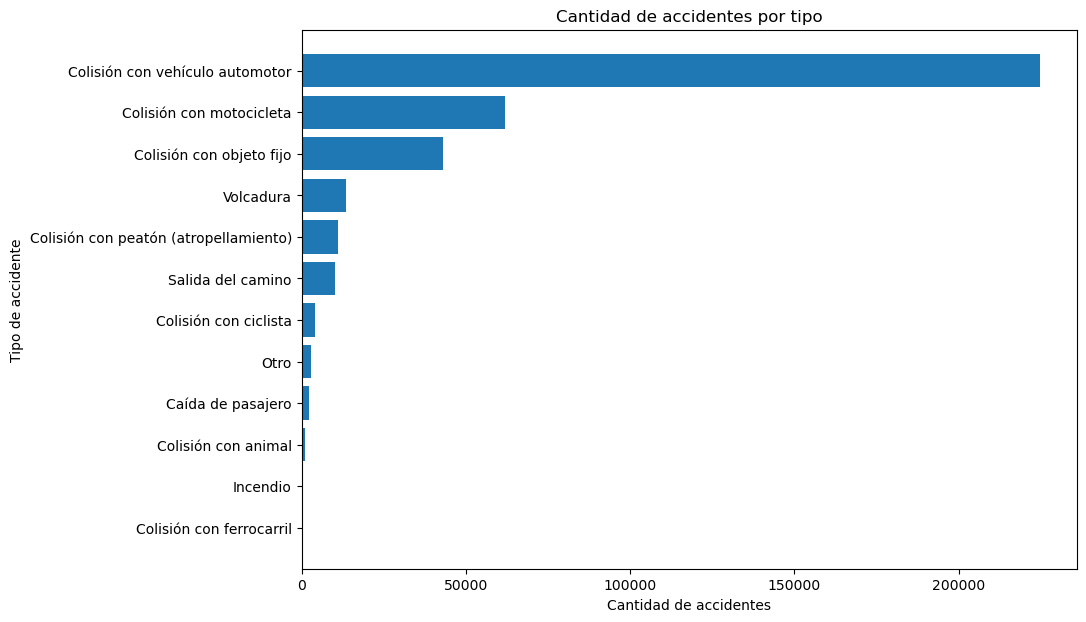
\includegraphics[width=0.88\textwidth]{figures/tipos_accidente.png}
    \caption{Cantidad de accidentes según el tipo de percance.}
\end{figure}

\begin{nota}
La causa presunta y la superficie de rodamiento aportan información adicional
sobre el contexto del evento.

\vspace{0.4em}
\begin{tabularx}{\textwidth}{L{4.2cm}rrY}
    \toprule
    \textbf{Variable y categoría} & \textbf{Accidentes} & \textbf{Porcentaje}
        & \textbf{Lectura} \\
    \midrule
    \code{CAUSAACCI}: conductor & 360,051 & 96.03\%
        & Categoría ampliamente dominante. \\
    \code{CAUSAACCI}: condición del camino & 5,991 & 1.60\%
        & Segunda causa presunta más frecuente. \\
    \code{CAUSAACCI}: falla del vehículo & 3,978 & 1.06\%
        & Frecuencia reducida respecto al conductor. \\
    \code{CAPAROD}: pavimentada & 368,913 & 98.39\%
        & Superficie registrada en la mayoría de los eventos. \\
    \code{CAPAROD}: no pavimentada & 6,036 & 1.61\%
        & Superficie minoritaria en el archivo. \\
    \bottomrule
\end{tabularx}

\vspace{0.4em}
\code{CAUSAACCI} representa una clasificación presunta registrada en el dataset,
no una demostración independiente de causalidad. De manera similar, la cantidad
de accidentes en superficies pavimentadas no demuestra que éstas sean más
peligrosas, pues el archivo no contiene medidas de exposición como longitud de
vialidades o número de desplazamientos.
\end{nota}

\subsection*{5.6 Vehículos involucrados}

\begin{nota}
Las trece columnas vehiculares indican cuántas unidades de cada categoría
participaron en un percance. No son variables excluyentes: un mismo accidente
puede involucrar automóviles, motocicletas u otros vehículos simultáneamente.
En la vista auxiliar se contabilizaron 710,403 vehículos, con un promedio de
1.89 por accidente.

\vspace{0.4em}
\begin{tabularx}{0.92\textwidth}{Yrrr}
    \toprule
    \textbf{Categoría} & \textbf{Vehículos} & \textbf{Porcentaje}
        & \textbf{Accidentes donde aparece} \\
    \midrule
    Automóvil & 436,681 & 61.47\% & 302,962 \\
    Motocicleta & 86,124 & 12.12\% & 80,101 \\
    Camioneta de pasajeros & 79,558 & 11.20\% & 69,664 \\
    Camioneta de carga & 51,106 & 7.19\% & 47,432 \\
    \bottomrule
\end{tabularx}
\end{nota}

\begin{figure}[H]
    \centering
    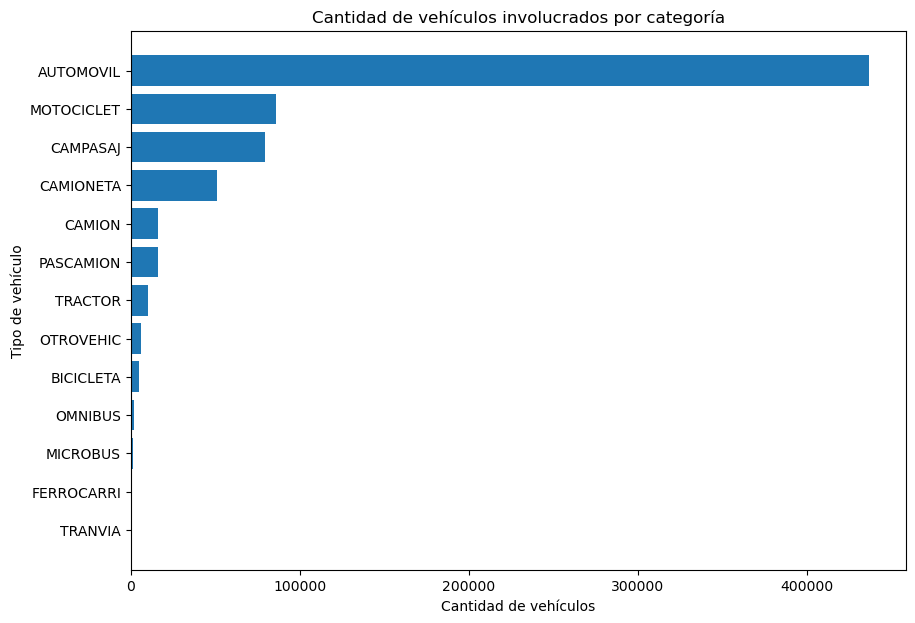
\includegraphics[width=0.84\textwidth]{figures/vehiculos_involucrados.png}
    \caption{Cantidad total de vehículos involucrados por categoría.}
\end{figure}

\begin{nota}
\begin{tabularx}{0.74\textwidth}{Yr}
    \toprule
    \textbf{Cantidad de vehículos por accidente} & \textbf{Accidentes} \\
    \midrule
    1 & 61,910 \\
    2 & 294,083 \\
    3 & 16,313 \\
    4 & 2,083 \\
    5 o más & 560 \\
    \bottomrule
\end{tabularx}

\vspace{0.4em}
La mayoría de los accidentes, aproximadamente el 78.43\%, involucra exactamente
dos vehículos.
\end{nota}

\subsection*{5.7 Información del conductor}

\begin{nota}
La exploración revisó las características disponibles del conductor presunto
responsable. En cuanto al sexo registrado, 278,004 accidentes corresponden a
hombres (74.14\%), 61,908 a mujeres (16.51\%) y 35,037 a casos en los que el
conductor se fugó (9.34\%).

\vspace{0.4em}
Antes de calcular estadísticas de edad fue necesario separar los códigos
especiales. Dentro de la vista auxiliar de accidentes, el valor 0 aparece en
35,037 registros y corresponde a conductores fugados, el valor 99 aparece en
61,564 registros y representa edad desconocida. Después de excluir ambos códigos
quedan 278,348 edades válidas entre 12 y 98 años. La media es de 37.85 años y la
mediana de 35 años, la mayor concentración se observa entre los 18 y 49 años.
\end{nota}

\begin{figure}[H]
    \centering
    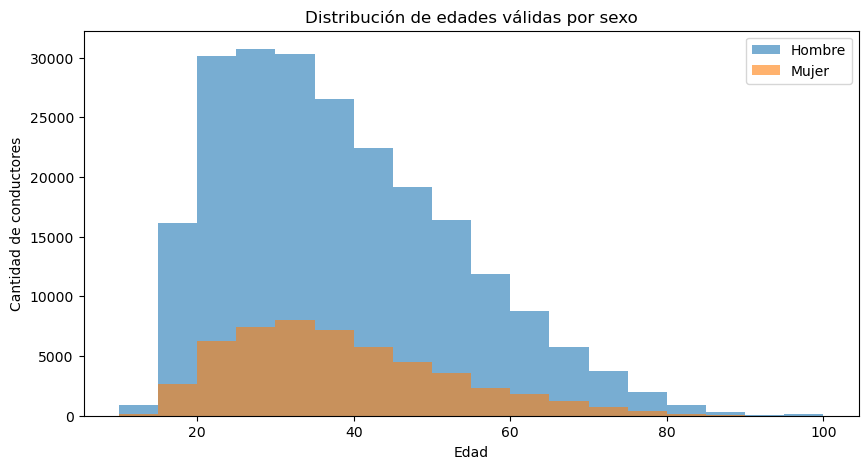
\includegraphics[width=0.82\textwidth]{figures/edades_validas_por_sexo.png}
    \caption{Distribución de edades válidas según el sexo registrado.}
\end{figure}

\begin{nota}
Las variables \code{ALIENTO} y \code{CINTURON} contienen una cantidad relevante
de casos desconocidos. Por ello conviene distinguir el porcentaje sobre todos
los accidentes del porcentaje calculado únicamente entre casos conocidos.

\vspace{0.4em}
\begin{tabularx}{\textwidth}{L{2.4cm}L{2.2cm}rrY}
    \toprule
    \textbf{Variable} & \textbf{Valor} & \textbf{Accidentes}
        & \textbf{Porcentaje} & \textbf{Entre casos conocidos} \\
    \midrule
    Aliento alcohólico & Sí & 15,915 & 4.24\% & 6.24\% \\
    Aliento alcohólico & No & 239,170 & 63.79\% & 93.76\% \\
    Aliento alcohólico & Se ignora & 119,864 & 31.97\% & No aplica \\
    \midrule
    Cinturón & Sí & 42,451 & 11.32\% & 49.51\% \\
    Cinturón & No & 43,285 & 11.54\% & 50.49\% \\
    Cinturón & Se ignora & 289,213 & 77.13\% & No aplica \\
    \bottomrule
\end{tabularx}

\vspace{0.4em}
En el caso de \code{ALIENTO}, la columna registra la presencia de aliento
alcohólico, pero no permite determinar el grado de consumo ni afirmar que el
alcohol causó el percance. Para \code{CINTURON}, la proporción de información
desconocida es particularmente alta y la variable sólo describe al conductor
presunto responsable, no al resto de ocupantes.
\end{nota}

\subsection*{5.8 Víctimas, severidad y estatus}

\begin{nota}
Las variables de víctimas contabilizan personas heridas y fallecidas según su
tipo de participación. Es importante distinguir estas cantidades del número de
accidentes, pues un mismo percance puede afectar a más de una persona.

\vspace{0.4em}
\begin{tabularx}{0.78\textwidth}{Yrr}
    \toprule
    \textbf{Tipo de persona} & \textbf{Fallecidas} & \textbf{Heridas} \\
    \midrule
    Conductores & 2,614 & 45,442 \\
    Pasajeros & 972 & 26,828 \\
    Peatones & 901 & 11,509 \\
    Ciclistas & 142 & 2,097 \\
    Otras personas & 27 & 104 \\
    \midrule
    \textbf{Total} & \textbf{4,656} & \textbf{85,980} \\
    \bottomrule
\end{tabularx}

\vspace{0.4em}
Los conductores concentran el mayor número de víctimas, seguidos por pasajeros y
peatones. En total, 4,188 accidentes registraron al menos una persona fallecida
y 64,845 incluyeron al menos una persona herida. Las columnas de víctimas no
especificadas tienen valor cero en todos los registros.
\end{nota}

\begin{figure}[H]
    \centering
    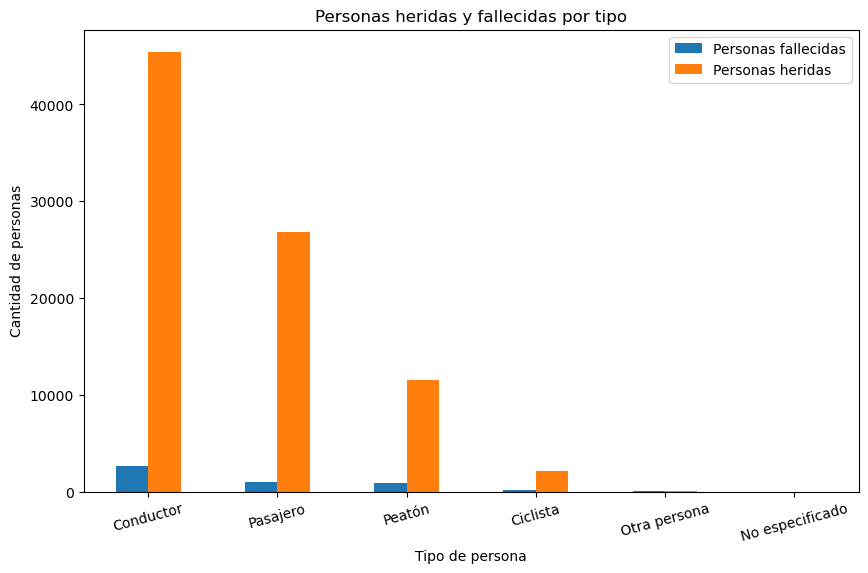
\includegraphics[width=0.68\textwidth]{figures/victimas_por_tipo.png}
    \caption{Personas heridas y fallecidas según su tipo de participación.}
\end{figure}

\begin{nota}
La variable \code{CLASACC} resume la severidad del accidente y será central para
el aprendizaje supervisado.

\vspace{0.4em}
\begin{tabularx}{0.7\textwidth}{Yrr}
    \toprule
    \textbf{Clasificación} & \textbf{Accidentes} & \textbf{Porcentaje} \\
    \midrule
    Sólo daños & 306,841 & 81.84\% \\
    No fatal & 63,920 & 17.05\% \\
    Fatal & 4,188 & 1.12\% \\
    \bottomrule
\end{tabularx}

\vspace{0.4em}
La cantidad de accidentes fatales coincide con los 4,188 eventos que registran
al menos una persona fallecida, de manera consistente con el diccionario
oficial. La distribución evidencia un desbalance considerable, especialmente
para la clase \code{Fatal}.
\end{nota}

\begin{figure}[H]
    \centering
    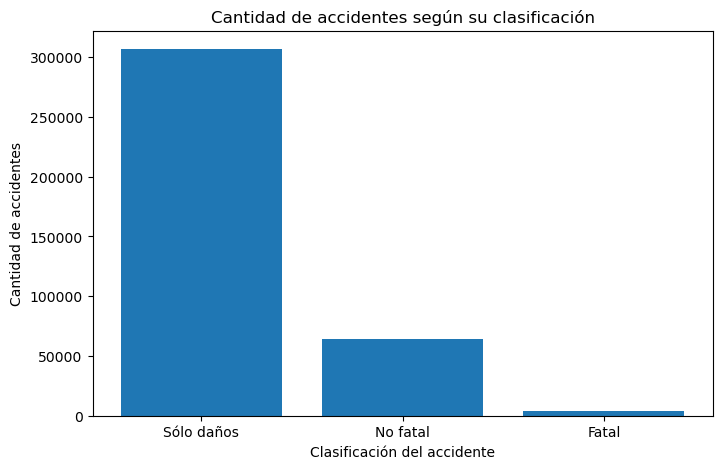
\includegraphics[width=0.72\textwidth]{figures/clasificacion_accidentes.png}
    \caption{Cantidad de accidentes según su clasificación de severidad.}
\end{figure}

\begin{nota}
Para el agrupamiento, \code{CLASACC} deberá excluirse de las variables de
entrada con el fin de formar grupos sin proporcionar previamente la severidad.
Por otra parte, \code{ESTATUS} indica el estado administrativo de las cifras:
356,109 accidentes corresponden a cifras definitivas (94.98\%) y 18,840 a cifras
corregidas (5.02\%). Como esta variable no describe el percance, se conserva
únicamente como referencia durante la exploración.
\end{nota}

\newpage
\subsection*{5.9 Limpieza y generación del dataset final}

\begin{nota}
A partir de los hallazgos anteriores se generó un nuevo archivo sin alterar el
CSV original. Las transformaciones se aplicaron de manera secuencial:

\vspace{0.4em}
\begin{tabularx}{\textwidth}{L{4cm}Y}
    \toprule
    \textbf{Transformación} & \textbf{Justificación y resultado} \\
    \midrule
    Eliminar duplicados exactos
        & Se retiraron 871 filas repetidas. El conjunto pasó de 390,627 a
          389,756 registros y no quedaron duplicados exactos. \\
    Eliminar columnas constantes
        & Se retiraron \code{COBERTURA}, \code{ANIO}, \code{NEMUERTO} y
          \code{NEHERIDO}, ya que no aportan variación para comparar registros
          ni entrenar modelos. \\
    Retirar \code{Certificado cero}
        & Se eliminaron 15,678 filas administrativas. Después de esta operación
          permanecen 374,078 accidentes. \\
    Separar códigos de edad
        & Se crearon \code{CONDUCTOR_FUGADO} y \code{EDAD_DESCONOCIDA}. Los
          códigos 0 y 99 se reemplazaron por valores nulos en \code{ID_EDAD}
          para evitar tratarlos como edades reales. \\
    Eliminar \code{ESTATUS}
        & Se retiró esta variable porque describe la publicación de las cifras,
          no las características del percance. \\
    \bottomrule
\end{tabularx}
\end{nota}

\begin{nota}
El resultado se exportó como \code{atus_anual_2024_limpio.csv}. Este archivo
contiene 374,078 filas y 42 columnas, conserva únicamente accidentes reales y no
presenta duplicados exactos.

\vspace{0.4em}
La diferencia entre los 374,949 accidentes de la vista auxiliar y los 374,078
registros del archivo final se debe a que la primera todavía conservaba filas
duplicadas. Al aplicar la limpieza, los únicos valores nulos restantes se
encuentran en \code{ID_EDAD}: 34,920 registros corresponden a conductores fugados
y 61,302 a edades desconocidas, para un total de 96,222 valores faltantes
intencionales. Es decir, permanecen 277,856 edades válidas.

\vspace{0.4em}

El dataset limpio constituye el punto de partida para el análisis estadístico,
la clasificación supervisada y el agrupamiento.
\end{nota}

\end{document}
